% !TeX spellcheck = en_US
\addscenariosection{1}{Cooperative scenario}{Titan's stronghold}{\images/Stronghold.png}

\begin{multicols*}{2}

\textbf{Author:} Invoceusse

\textbf{Source:} \href{https://discord.com/channels/740870068178649108/1219333721019256943}{Archon Studio Discord}

\subsection*{\MakeUppercase{Scenario length}}

This scenario plays out over 16 rounds. (15 in impossible)

\subsection*{\MakeUppercase{Player setup}}

\textbf{Player count:} 1 - 6

\textbf{Starting Resources:} 30 \svg{gold}, 8 \svg{building_materials}, 2 \svg{valuables}

\textbf{Starting Income:} 10 \svg{gold}, 2 \svg{building_materials}, 1 \svg{valuables}

\textbf{Starting Units:} 
    A Pack of \svg{bronze} units of your choice.
    A Few \svg{bronze} units of your choice.

\textbf{Town Buildings:} nothing

\subsection*{\MakeUppercase{Map setup}}

Take the following Map tiles and set them up as shown in the scenario map layout: (P for number of player)

\textbf{(1*P) Starting Map tile (I)}
\begin{itemize}
    \item Starting Tiles of your chosen factions.
    \item Ignore all of their yellow line.
\end{itemize}

\textbf{(2*P) × Far Map tile (II-III)}

\textbf{(2*P) × Near Map tile (IV-V)}

\textbf{(1*P) + 1 × Center Map tile (VI-VII)}

If you don't have enough VI-VII tile you can use another for tile near to tile I.
The center of this tile is the Titans' Stronghold.

\columnbreak

\subsection*{\MakeUppercase{Win conditions}}

\textbf{Win:}
\begin{itemize}
	\item Kill all unit in the Titans' Stronghold (the center of tile VI-VII next to the tiles I)
\end{itemize}

\subsection*{\MakeUppercase{Timed events}}

\textbf{4$^{th}$, 8$^{th}$ and 12$^{th}$ Round:}
\begin{itemize}
	\item Remove black cubes from windmills, water wheels and mystical gardens.
\end{itemize}

\subsection*{\MakeUppercase{The story}}

TODO \end{multicols*}

\newpage

\subsection*{\MakeUppercase{Additional rules}}

\begin{itemize}
	\item Remember : the center of tile VI-VII next to all I, is the Titans' Stronghold.
	\item nobody can enter the titans' Stronghold before all other VII battle are flagged by any player.
	\item After defeating a level VII neutral army, instead of resolving field the player chooses an option three times from the following list (an option may be chosen multiple times):
	\begin{itemize}
		\item Another player (you choose) gains 5 gold
		\item Another player (you choose) gains 2 building materials
		\item Another player (you choose) gains 1 valuable
	\end{itemize}
	Then flag the VII with faction cube.
	(In solo play : no bonus!)
	\item Ignore all yellow line in tiles I.
	\item You can use your build token to give your resources to another player.
	\item Two player can use your build token for exchange artifacts and/or spells.
	\item Whenever a player visits an Obelisk, that player rolls one tresure dice and one resource dice, chooses one of the dice and resolves its outcome dice.
	\item When all VII (not includ the titans' Stronghold) are flagged, randomly draw and shuffle the following (next page) number of neutral Unit cards from each of their corresponding decks to create a separate deck of neutral Units for the titans' Stronghold (The deck of titans' Stronghold is sometimes cut in two because otherwise certain scenarios are impossible to implement with the cards of certain extensions.)
	\item Any time a Hero enters the titans' Stronghold they draw 5 cards from the Titans' Stronghold deck instead of drawing them from the Neutral Unit card decks. The units are placed on the Combat board (see page 29, “Neutral Unit Setup” in the Core Rulebook). Players attempt to beat the units they find at the Titans' Stronghold. Any Neutral Units defeated during Combat in the Titans' Stronghold are returned to their respective Neutral Unit decks instead of Titans' Stronghold deck. Any Neutral Units surviving Combat at the Titans' Stronghold are shuffled back into the Titans' Stronghold deck. If there are not enough Unit cards in this deck, draw as many Unit cards as there are and place them on the Combat board.
	\item Combat in the Titans' Stronghold now costs 1 MP to extend per Combat round, just like Combat against non-Azure tier units.
	\item Additionally, no player can:\linebreak
	a) Attack other Heroes.\linebreak
	b) Capture a Mine or Settlement that is already controlled.
\end{itemize}



\newpage

\hommtable[]{27}{
  \centering
  \medskip
  \textbf{Strength of Titans' Stronghold Armies}\\
  \bigskip

  \newcommand{\bronze}[0]{\svg[12]{bronze}}
  \newcommand{\silver}[0]{\svg[12]{silver}}
  \newcommand{\golden}[0]{\svg[12]{golden}}
  \newcommand{\azure}[0]{\svg[12]{azure}}

  \begin{tabularx}{\linewidth}{p{0.15\linewidth}XXXX} & \darkcell{Easy} & \darkcell{Normal} & \darkcell{Hard} & \darkcell{Impossible}\\
    \darkcell[1.4]{1 player} 
        & \lightcell[1.4]{3\bronze 2\silver 1\golden 1\azure}
        & \lightcell[1.4]{2\bronze 2\silver 2\golden 1\azure}
        & \lightcell[1.4]{2\bronze 2\silver 2\golden 2\azure}
        & \lightcell[1.4]{1\bronze 2\silver 2\golden 3\azure}\\
    \darkcell[1.4]{2 players} 
	    & \lightcell[1.4]{5\bronze 5\silver 3\golden 1\azure}
	    & \lightcell[1.4]{4\bronze 5\silver 3\golden 2\azure}
	    & \lightcell[1.4]{2\bronze 5\silver 5\golden 3\azure}
	    & \lightcell[1.4]{1\bronze 5\silver 7\golden 4\azure}\\
    \darkcell[1.4]{3 players} 
        & \lightcell[1.4]{8\bronze 7\silver 4\golden 2\azure}
        & \lightcell[1.4]{6\bronze 7\silver 5\golden 3\azure}
        & \lightcell[1.4]{2\bronze 3\silver 4\golden 3\azure \linebreak
        	Then\linebreak 
        	2\bronze 4\silver 3\golden 2\azure}
        & \lightcell[1.4]{1\bronze 3\silver 5\golden 3\azure \linebreak
        	Then\linebreak 
        	1\bronze 4\silver 5\golden 3\azure}\\
    \darkcell[1.4]{4 players} 
        & \lightcell[1.4]{10\bronze 10\silver 6\golden 2\azure}
        & \lightcell[1.4]{8\bronze 10\silver 6\golden 4\azure}
        & \lightcell[1.4]{2\bronze 5\silver 5\golden 3\azure \linebreak
        	Then\linebreak 
        	2\bronze 5\silver 5\golden 3\azure}
        & \lightcell[1.4]{1\bronze 5\silver 7\golden 4\azure \linebreak
        	Then\linebreak 
        	1\bronze 5\silver 7\golden 4\azure}\\
	\darkcell[1.4]{5 players} 
	  	& \lightcell[1.4]{6\bronze 6\silver 4\golden 1\azure \linebreak
	  		Then\linebreak 
	  		7\bronze 6\silver 3\golden 2\azure}
	  	& \lightcell[1.4]{5\bronze 6\silver 4\golden 2\azure \linebreak
	  		Then\linebreak 
	  		5\bronze 6\silver 4\golden 3\azure}
	  	& \lightcell[1.4]{3\bronze 6\silver 6\golden 4\azure \linebreak
	  		Then\linebreak 
	  		3\bronze 6\silver 6\golden 4\azure}
	  	& \lightcell[1.4]{1\bronze 6\silver 8\golden 6\azure \linebreak
	  		Then\linebreak 
	  		2\bronze 6\silver 8\golden 5\azure}\\
	\darkcell[1.4]{6 players} 
	  	& \lightcell[1.4]{8\bronze 8\silver 4\golden 1\azure \linebreak
	  		Then\linebreak 
	  		7\bronze 7\silver 5\golden 2\azure}
	  	& \lightcell[1.4]{6\bronze 8\silver 4\golden 3\azure \linebreak
	  		Then\linebreak 
	  		6\bronze 7\silver 5\golden 3\azure}
	  	& \lightcell[1.4]{3\bronze 8\silver 7\golden 5\azure \linebreak
	  		Then\linebreak 
	  		3\bronze 7\silver 8\golden 4\azure}
	  	& \lightcell[1.4]{3\bronze 7\silver 11\golden 6\azure \linebreak
	  		Then\linebreak 
	  		3\bronze 8\silver 10\golden 6\azure}\\
  \end{tabularx}
}

\vspace{3em}

\center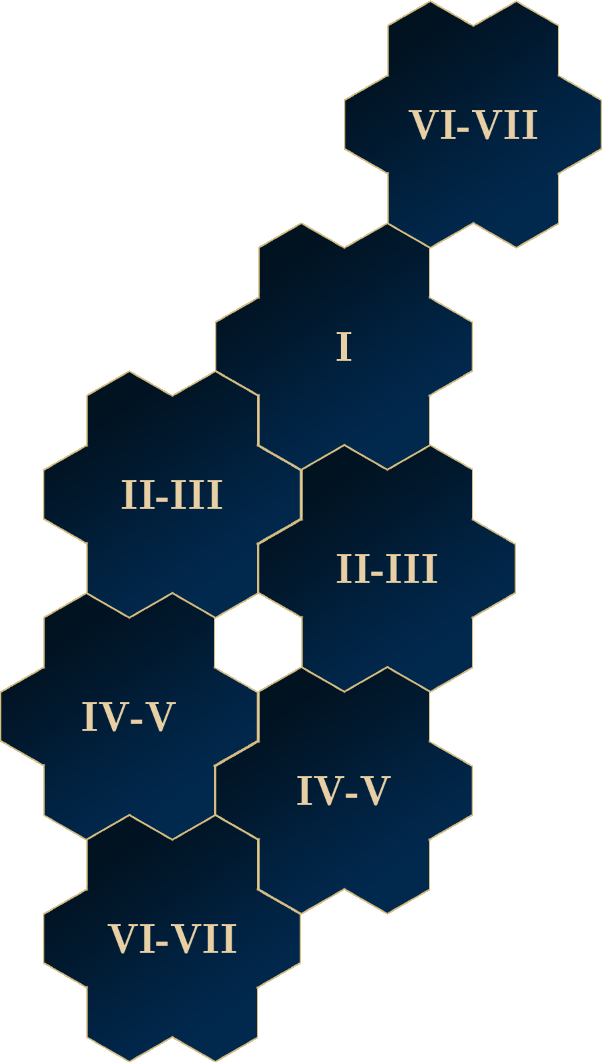
\includegraphics[width=0.2\paperwidth]{\_assets/maps/titans-1.png}
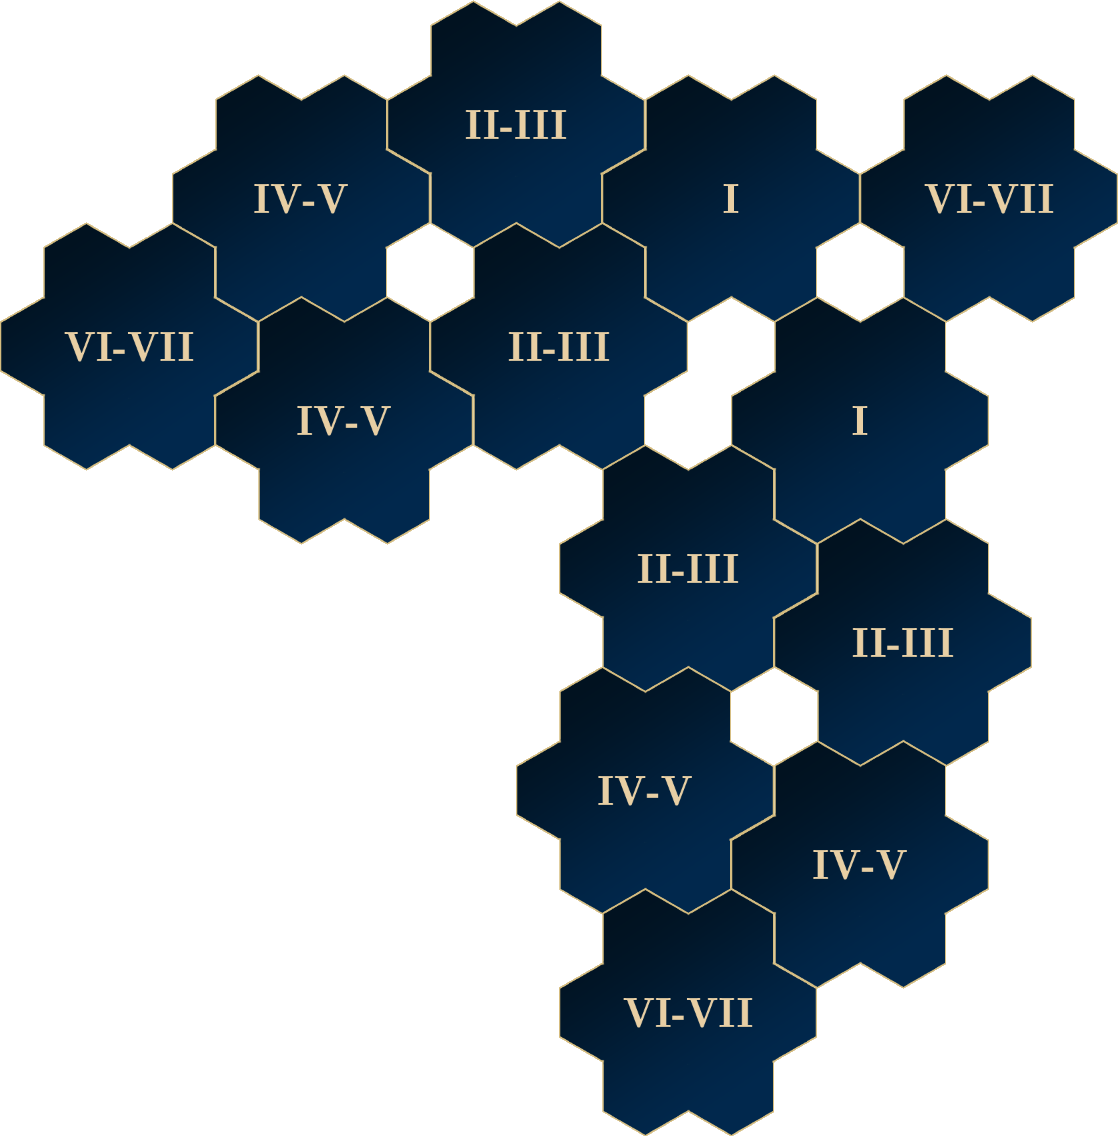
\includegraphics[width=0.4\paperwidth]{\_assets/maps/titans-2.png}
\center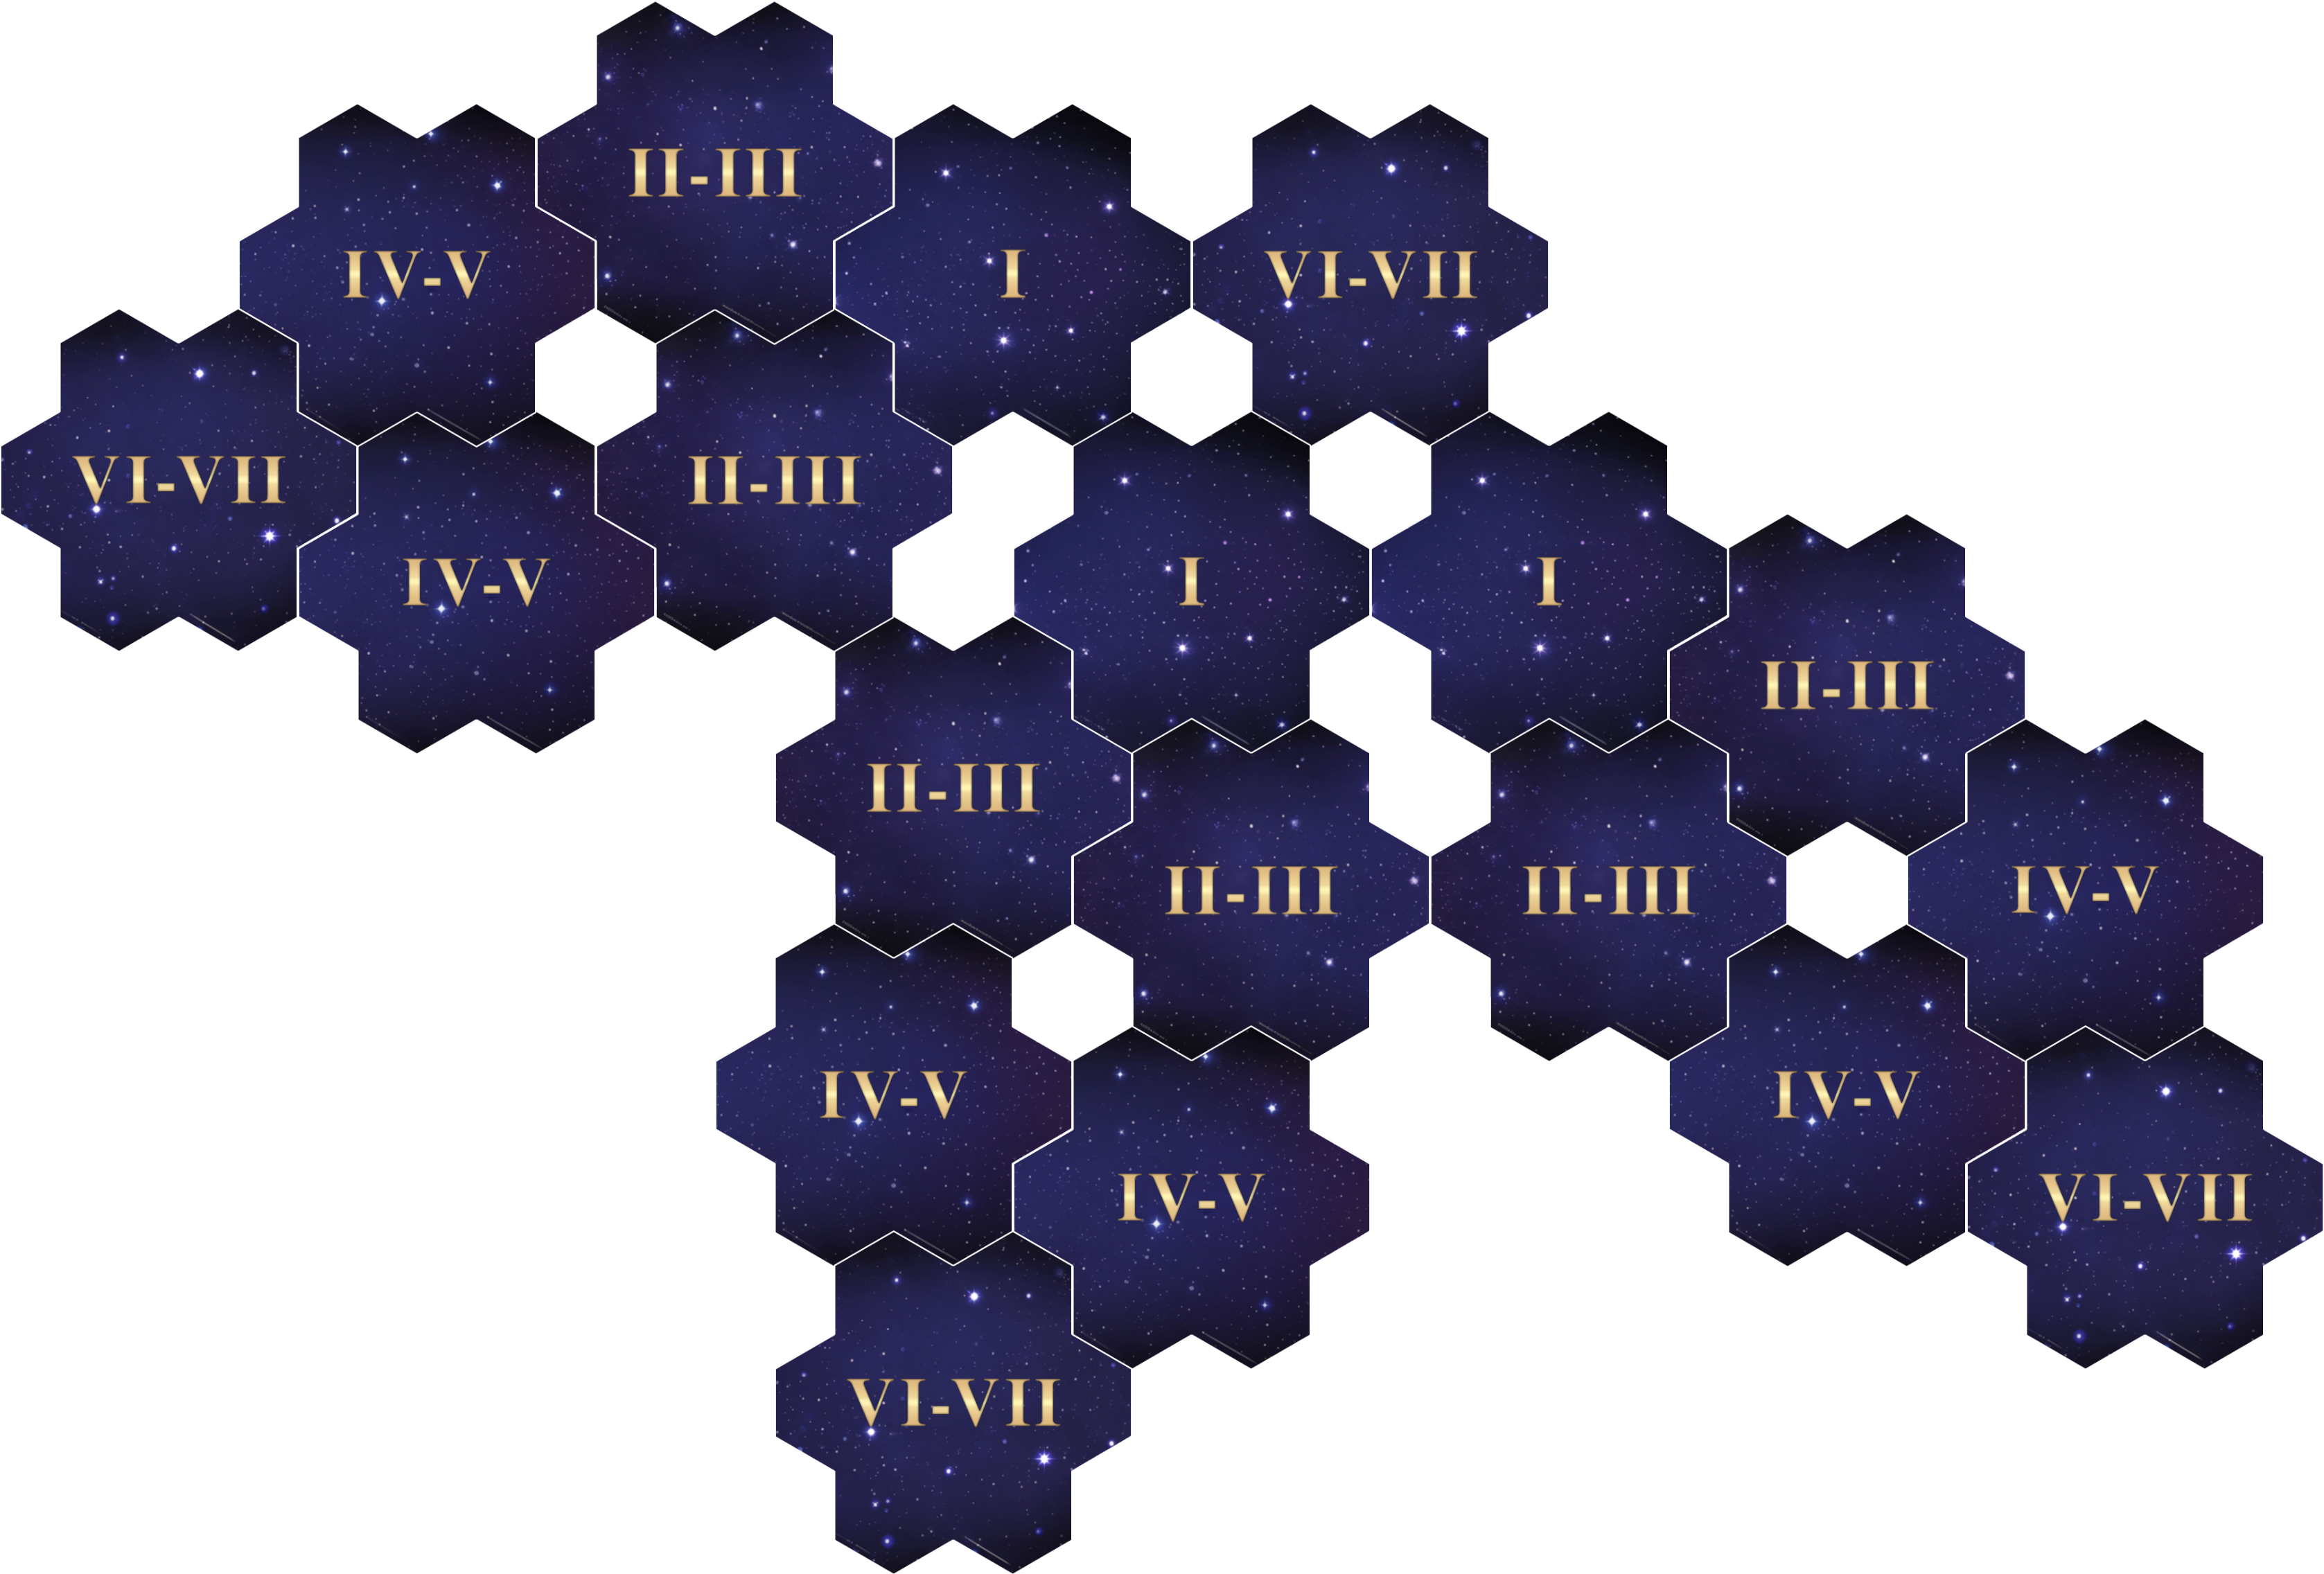
\includegraphics[width=0.4\paperwidth]{\_assets/maps/titans-3.png}
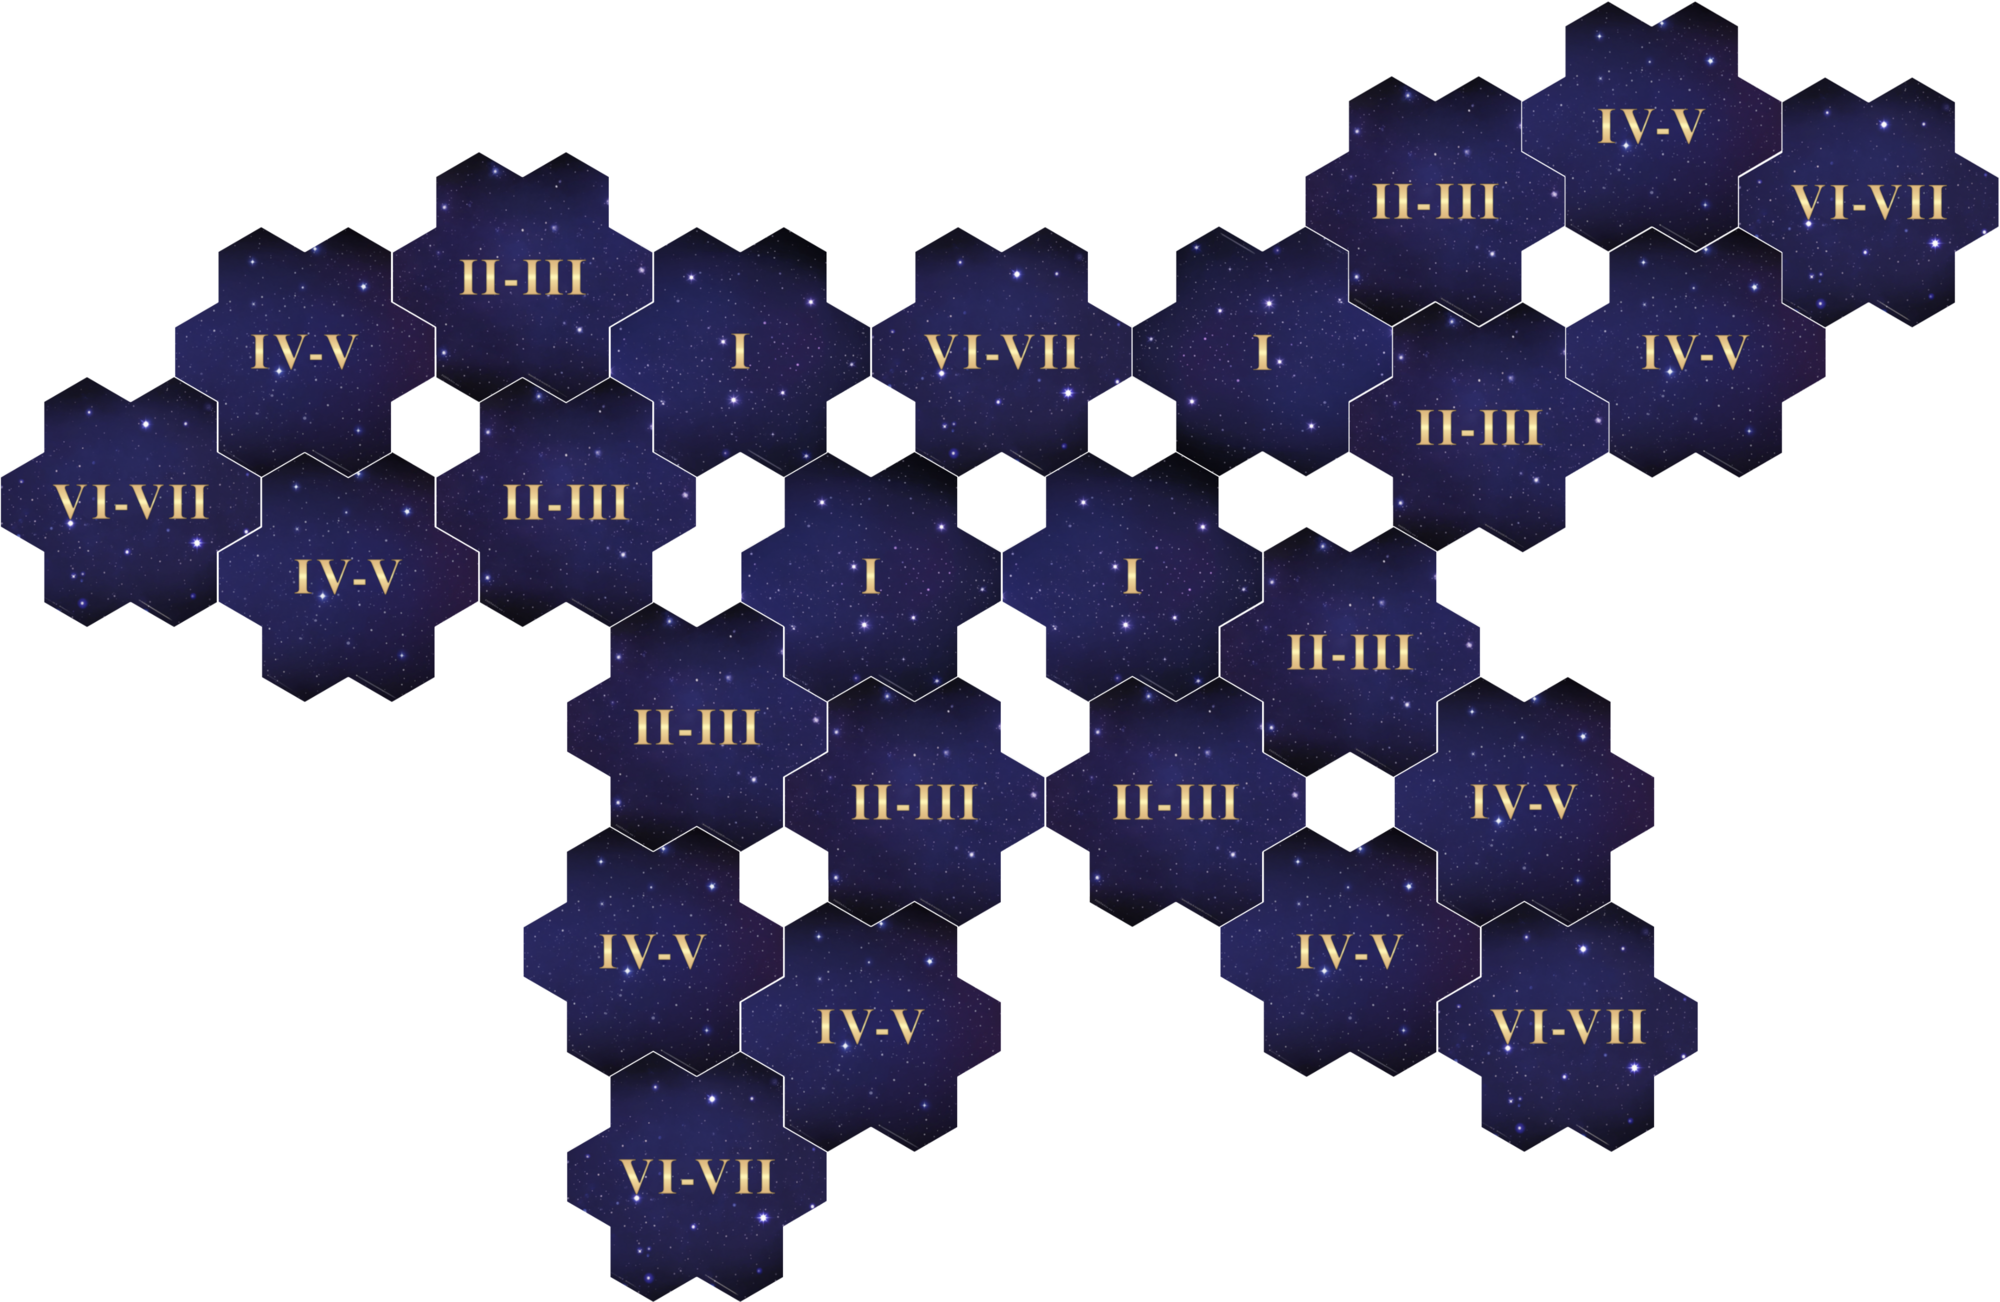
\includegraphics[width=0.4\paperwidth]{\_assets/maps/titans-4.png}
\center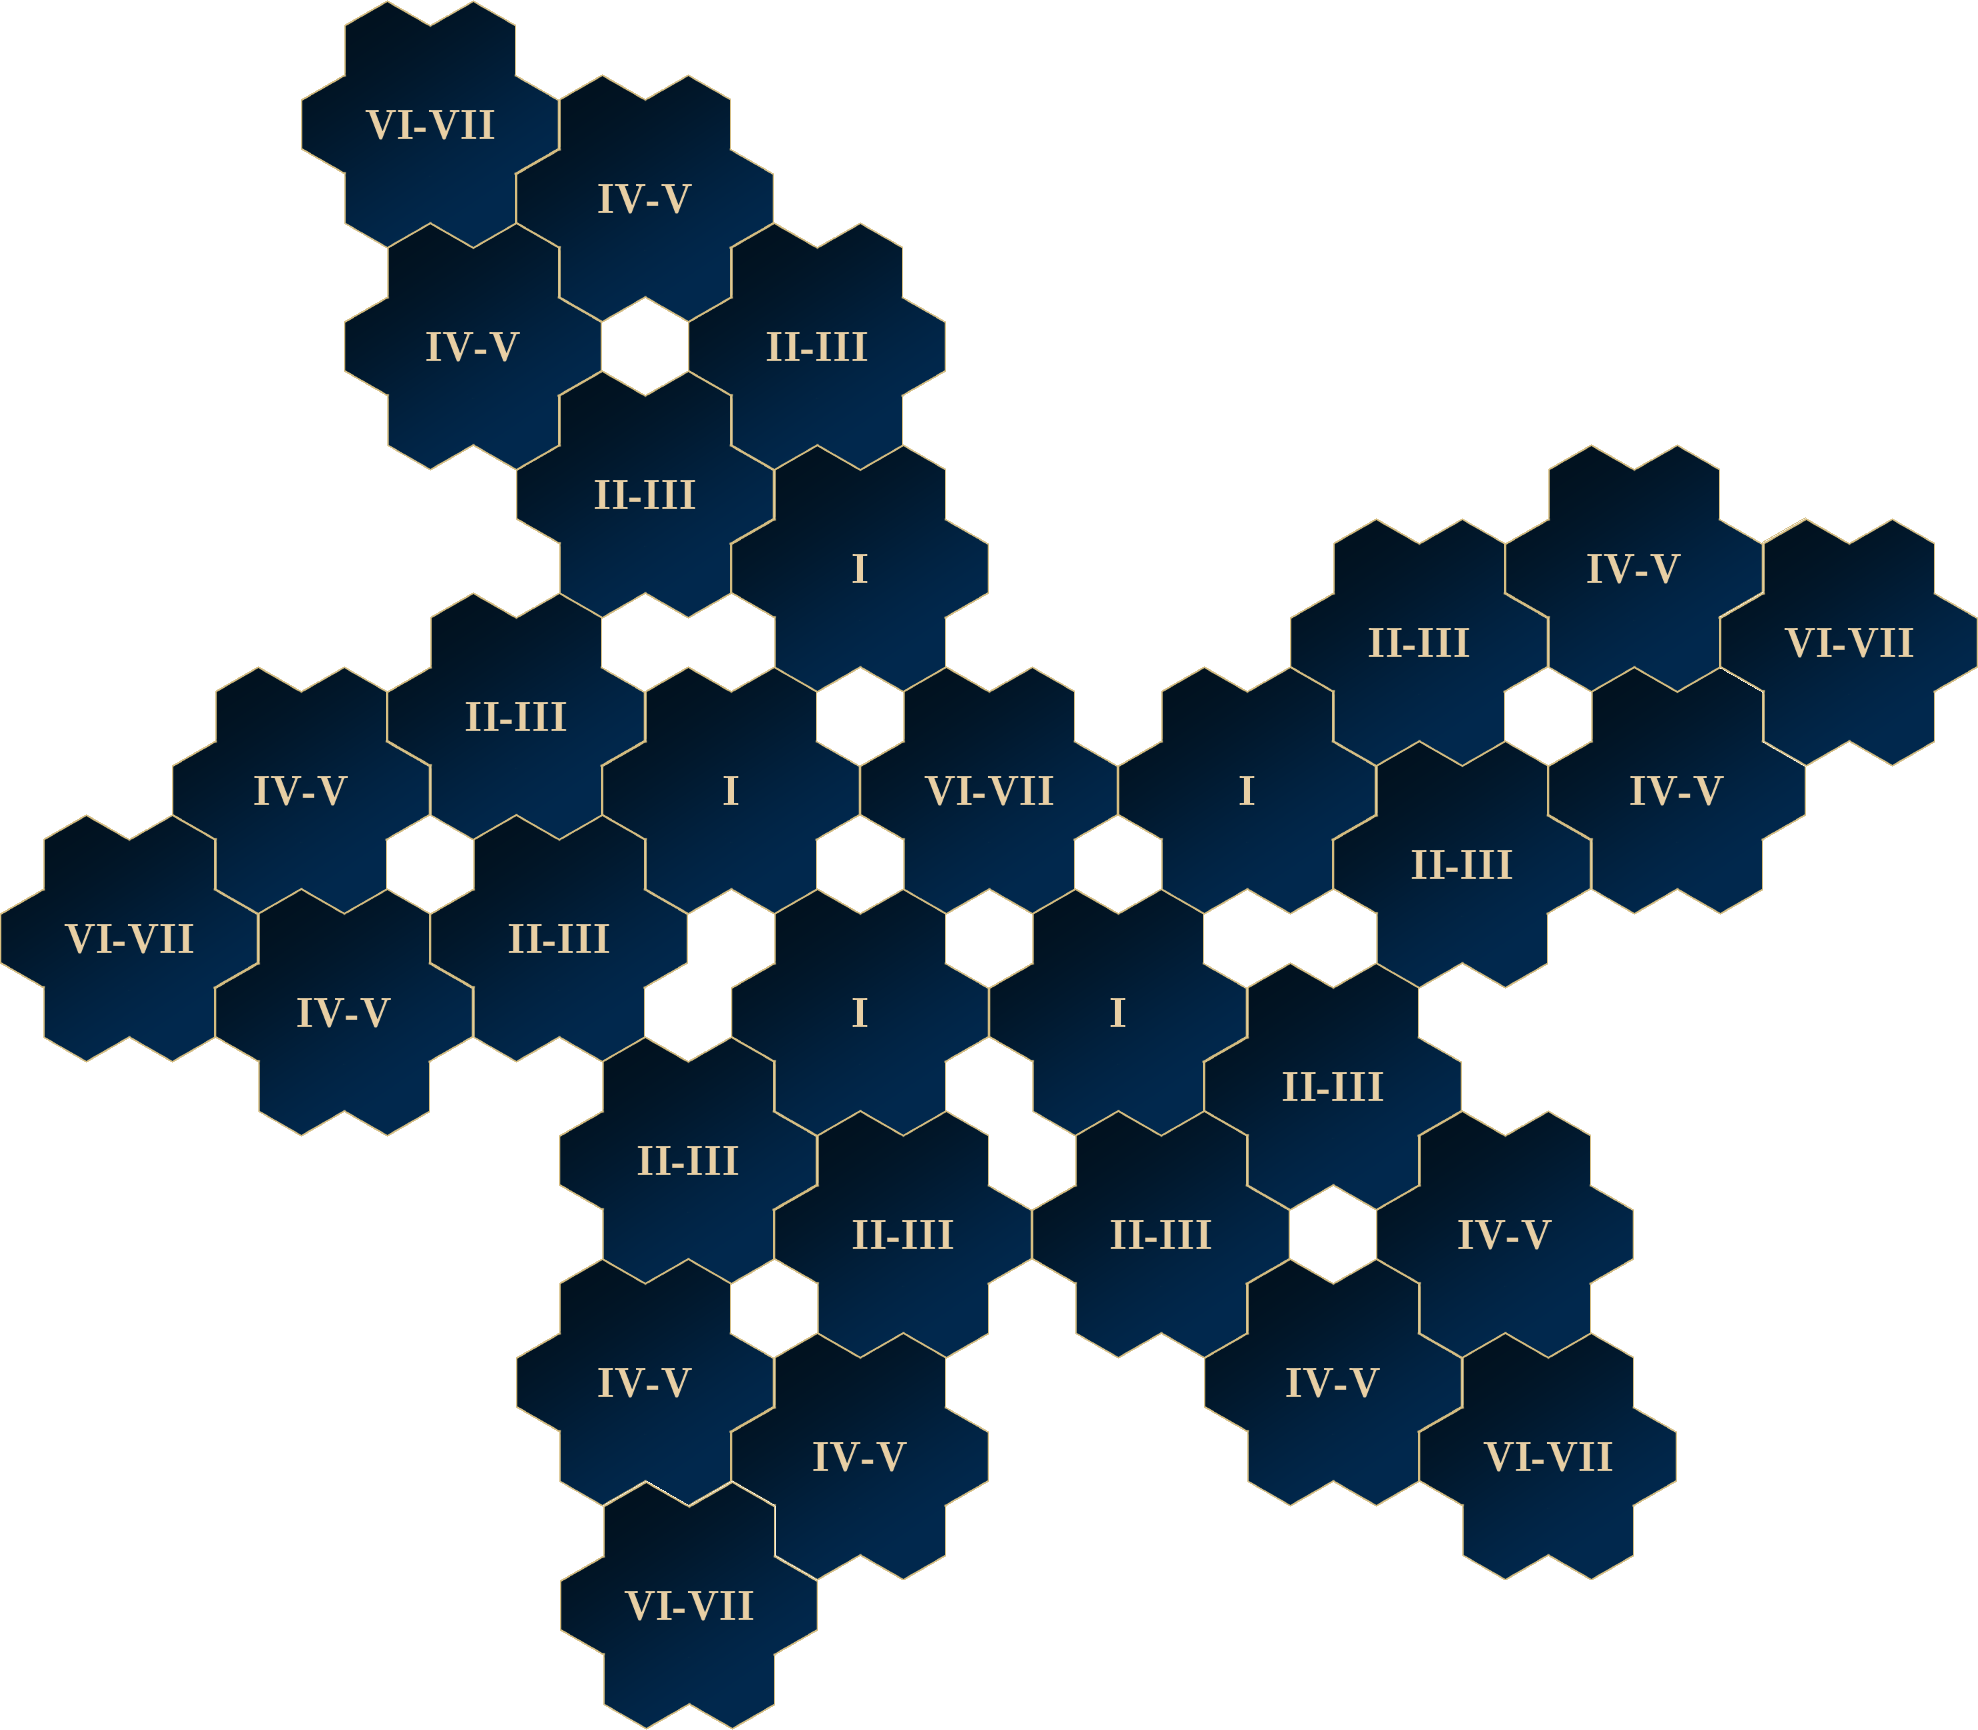
\includegraphics[width=0.4\paperwidth]{\_assets/maps/titans-5.png}
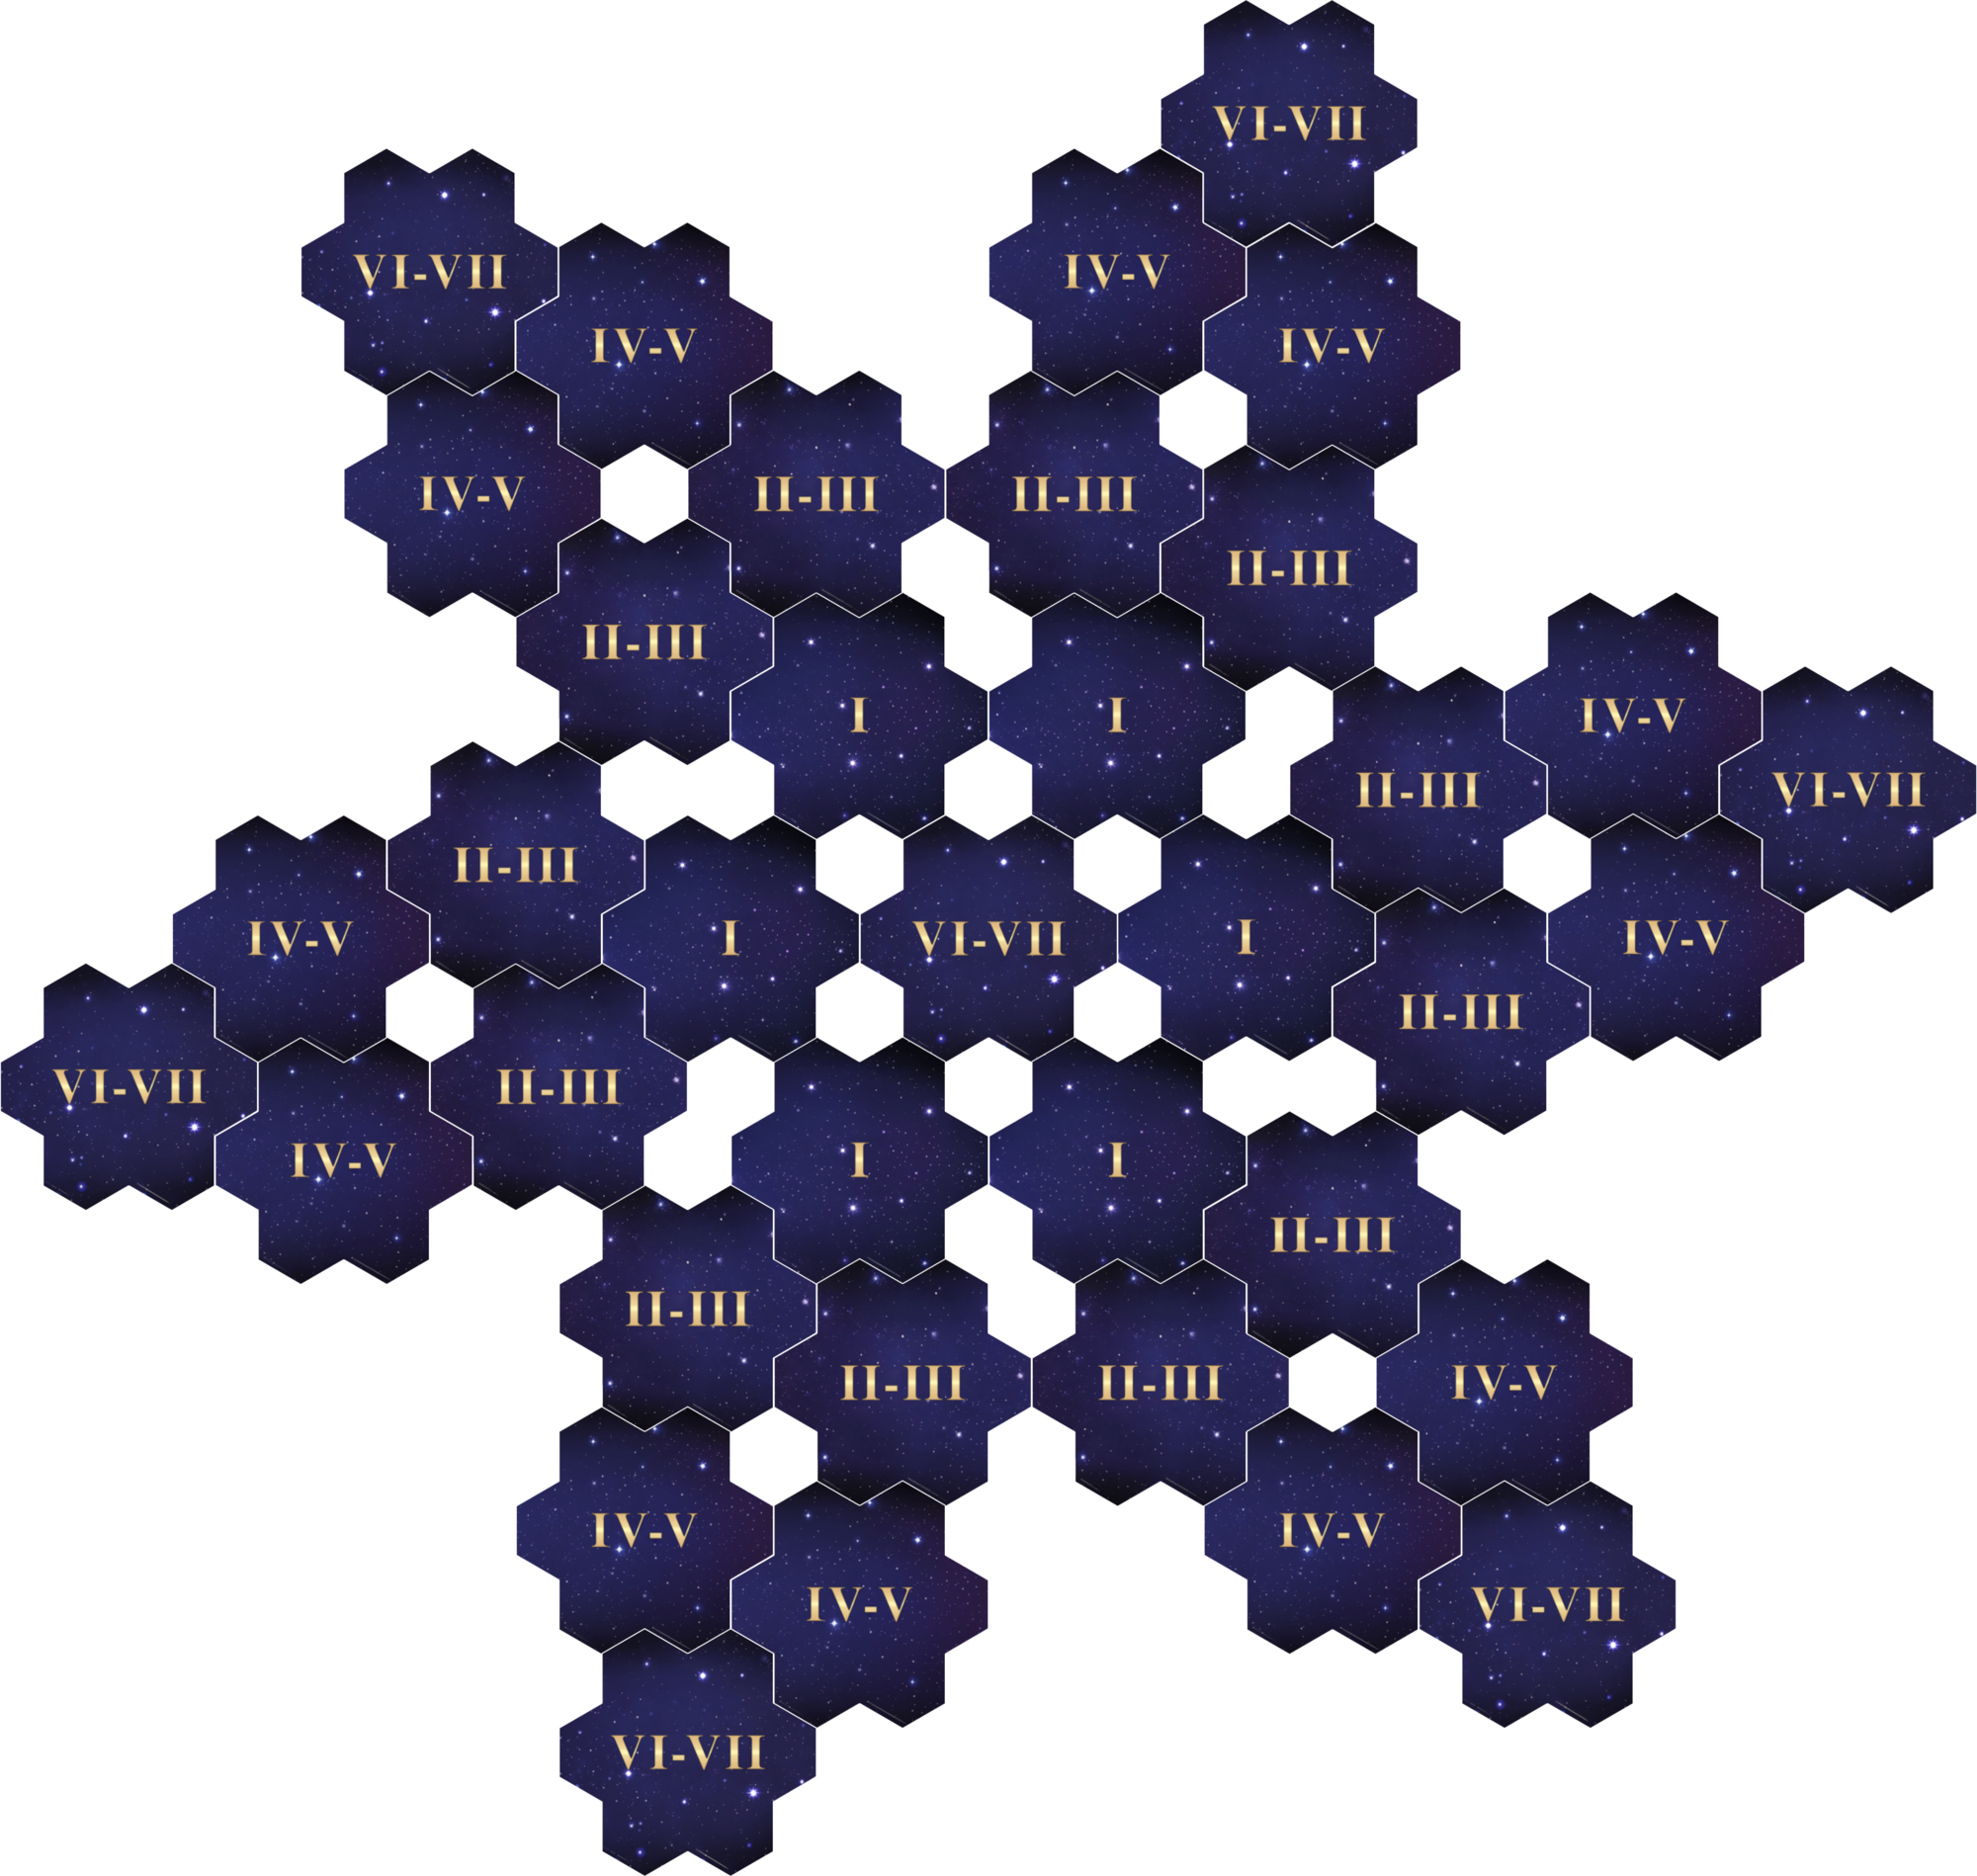
\includegraphics[width=0.4\paperwidth]{\_assets/maps/titans-6.png}
